\subsection{Multicore Models including Contention with Constraints}

\label{subsubsection: multicore evaluation with constraints}

In this section, we validate multicore models of REPP by predicting performance and power
at the hardware settings DVFS states and Cl-States (Section~\ref{subsec: algo}), and then
select a configuration to satisfy the user provided constraint.  This constraint is
defined as either delivering a minimum performance, or not violating a power target.
Therefore, to satisfy either of these constraints, REPP provides a dynamic configuration
selector.


\subsubsection{REPP Configuration Selector}
\label{subsubsec: config selec}
\nomenclature[g-omega]{$\omega$}{The performance or power constraint per core}


\looseness -1 Modern data centres have power constraints (e.g., power capping) and run
multiple application instances with different performance constraints.  This requires an
algorithm to select a configuration per core such that the performance and power
constraints are met per core and/or per application, given by $\omega$. To ensure that
these constraints are met, REPP dynamically selects a configuration per core every
\SI{250}{\milli\second} by performing a linear search for the DVFS state that is the
nearest to the given constraint; next, REPP selects the Cl-State for the given DVFS
state that satisfies the constraint. This selected configuration, DVFS state, Cl-State, is
used to ensure that the constraint is met for each interval. 

Figure~\ref{fig: repphconfigselec} demonstrates a configuration selector to satisfy a user
defined power or performance constraint of \SI{40}{\percent}. We build one such model to
predict performance or power per core. The single-core models predict performance and
power for each configuration available in the 2-D space of DVFS state and Cl-State. We
repeat the aforementioned process for each core at the same time.


\begin{figure}
    \centering
    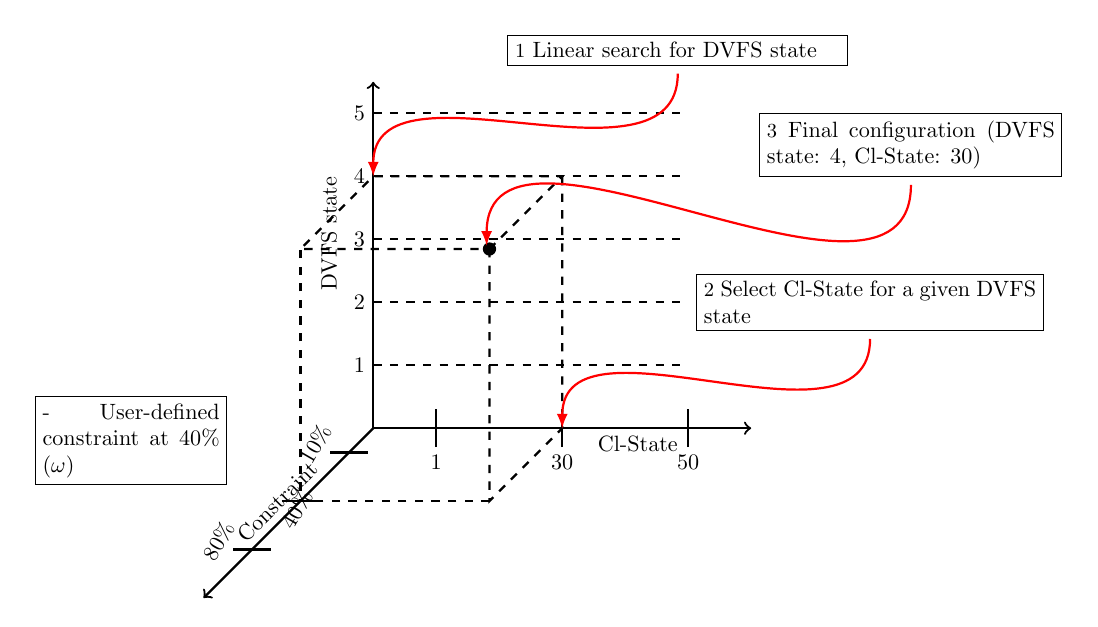
\begin{tikzpicture}[thick,scale=0.8, every node/.style={transform shape}]


    \draw[->] (0,0,0)-- node[pos=.7,below] {Cl-State} ++(6,0,0);
    \draw[->] (0,0,0)--++(0,5.5,0) node[pos=.75, left=7mm,rotate=90]{DVFS state};% ++(0,0,0);
    \draw[->] (0,0,0)--++(0,0,7) node[midway, sloped, above] {Constraint};

    \draw[-] (1,-.3,0) node[below]{1}--(1,.3,0);
    \draw[-] (3,-.3,0) node[below]{30}--(3,.3,0);
    \draw[-] (5,-.3,0) node[below]{50}--(5,.3,0);

    \draw[-] (-0.3,0,1) node[above, rotate=60]{10\%}--(0.3,0,1);
    \draw[-] (-0.3,0,3) node[below, rotate=60]{40\%}--(0.3,0,3);
    \draw[-] (-0.3,0,5) node[above, rotate=60]{80\%}--(0.3,0,5);

    \fill (3,4,3) circle(3pt);

    \draw[dashed] (3,4,3)--(3,4,0)--(0,4,0)--(0,4,3)--cycle;
    \draw[dashed] (3,4,3)--(3,0,3)--(3,0,0)--(3,4,0);
    \draw[dashed] (3,0,3)--(0,0,3)--(0,4,3);


    \foreach \i in {1,2,...,5}
       \draw[dashed] (0,\i,0) node[left] {\i} --++(5,0,0);

    \node [anchor=west] (note2) at (2,6) {
        \fbox{\begin{minipage}{14.7em}
            {\small \circled{1}} Linear search for DVFS state
    \end{minipage}}};

    \node [anchor=west] (notex) at (5,2) {
        \fbox{\begin{minipage}{15em}
            {\small \circled{2}} Select Cl-State for a given DVFS state
    \end{minipage}}};

    \node [anchor=west] (notea) at (-5.5,-0.2) {
        \fbox{\begin{minipage}{8.0em}
            - User-defined constraint at 40\% ($\omega$)
    \end{minipage}}};

    \node [anchor=west] (noteaa) at (6,4.5) {
        \fbox{\begin{minipage}{13em}
            {\small \circled{3}} Final configuration (DVFS state: 4, Cl-State: 30)
    \end{minipage}}};

    \draw [-latex, thick, red] (note2) to[out=270, in=90] (0,4);
    \draw [-latex, thick, red] (notex) to[out=270, in=90] (3,0);
    \draw [-latex, thick, red] (noteaa) to[out=270, in=90] (1.8,2.9);

    \end{tikzpicture}
    \caption[REPP configuration selector]{\captitle{REPP configuration selector.} An example of the configuration selector to satisfy a user-defined constraint of \SI{40}{\percent} for either power or performance for a single-core.}
\usetikzlibrary{positioning}
\label{fig: repphconfigselec}
\end{figure}


In our study, the performance and power constraints are given at a system level. These
constraints are  distributed  homogeneously across all cores. For example, if an AMD
server can only consume \SI{600}{\watt}, that power constraint is distributed
\SI{25}{\percent} per core, allowing each core to consume \SI{150}{\watt} (it would be
\SI{50}{\percent} on ARM). In this aforementioned example, $\omega$ is \SI{150}{\watt}.
At runtime, for the spawned applications, REPP samples application behaviour
periodically and uses the models built to predict performance and power at all
configurations. REPP then selects the configuration for each interval to satisfy the
local constraint.


\subsubsection{Experiments}
\label{subsubsec: experiments repph}

We perform two types of experiments: one for validating the power capping mechanism and
the other for delivering a minimum performance. We define two input parameters: (a)
frequency of change, and (b) $\chi$, which represents load or power.  The average load
offered by the applications is constant between two load changes, which can occur every
\textbf{load\_change interval} (1, 6, or 9 seconds), based on a \textbf{change\_factor},
as follows.  Load starts at a minimum, and varies by multiplying load by change\_factor
$\tau$ until it reaches a maximum load $\chi_{\mathit{max}}$; thereafter, the load is
multiplied by the negative value of change\_factor until it reaches the minimum
$\chi_{\mathit{min}}$.

\looseness -1 The values of change\_factor tested were \SI{20}{\percent} (\textbf{Low}),
\SI{35}{\percent} (\textbf{Mid}), and \SI{50}{\percent} (\textbf{High}). The minimum load
is defined as the sum of smallest IPS for all four applications running at minimum
frequency; similarly, maximum load is the sum of highest IPS for all four applications at
maximum frequency. In another set of experiments, we change the power consumed by the
workload similar to the load offered by the workload. 

\looseness -1 Mathematically, the experiment conducted for a load\_change interval 1 can
be represented as follows: In Equation~\ref{eq: topofcurve}, $\psi$ represents the number
of datapoints before the maximum load/power ($\chi_{\mathit{max}}$), and in
Equation~\ref{eq: eachterm}, $\chi(\kappa)$ shows the datapoint $\kappa$ in the sequence.

\vspace{0.2cm}

\begin{equation}
    \label{eq: topofcurve}
    \psi = \Bigl\lfloor\dfrac{\log(\chi_{\mathit{max}}/\chi_{\mathit{min}})}{\log(1+\tau)}\Bigr\rfloor\qquad                   
\end{equation}

\vspace{0.2cm}

\begin{equation}
    \label{eq: eachterm}
    \chi(\kappa) =
\left\{
    \begin{array}{ll}
        \chi_{\mathit{min}} \times (1+\tau)^{n}  & 0 \leq n \leq \psi\\
        \chi_{\mathit{max}} \times (1+\tau)^{2\psi-n}  & \psi < n \leq 2\psi
    \end{array}
\right.                    
\end{equation} 


\vspace{0.2cm}

\nomenclature[g-psi]{$\psi$}{Number of datapoints before the peak in a step-wise monotonic function}
\nomenclature[g-tau]{$\tau$}{Change\_factor for the step-wise monotonic function}
\nomenclature[g-chi]{$\chi$}{Load (IPS) or power in a step-wise monotonic function}
\nomenclature[g-chi]{$\chi(\kappa)$}{$\kappa^{th}$ element in the data sequence for either load or power}
\nomenclature[g-chi]{$\chi(min), \chi(max)$}{The minimum, maximum value of load or power}


The error occurs when REPP selects a configuration that makes the application fall short
of the minimum required performance (or exceed the maximum power requirement) in a given
mapping interval.

We ran ten experiments for power and ten for performance.  Nine of them come from the
combinations of the two parameters (frequency of change and load/power) described above;
the tenth comes from a \textbf{Random} setting within fixed boundaries of either power or
performance. Selecting a broad spectrum of load (or power) and frequency of change allowed
us to validate REPP across multiple combination of configurations at runtime. 

\subsection*{Evaluation of the Multicore Models with Constraints}
\label{subsubsec: eval repph}

We present the results, and evaluate REPP when predicting performance and power on
multicore processors by selecting a configuration in a single step to meet power and
performance requirements for 35 multiprogrammed workloads across 20 experiments (ten for
power and ten for performance).  The prediction error is computed over a period of 400
seconds for all DVFS states and Cl-States. The error metric indicates that the constraint
was violated by that amount, which occurs when REPP selects a configuration that makes
the application fall short of the minimum required performance (or exceed the maximum
power requirement) in a given mapping interval. 

\begin{figure}[t]
   \centering
    \begin{subfigure}{\textwidth}
        \centering
        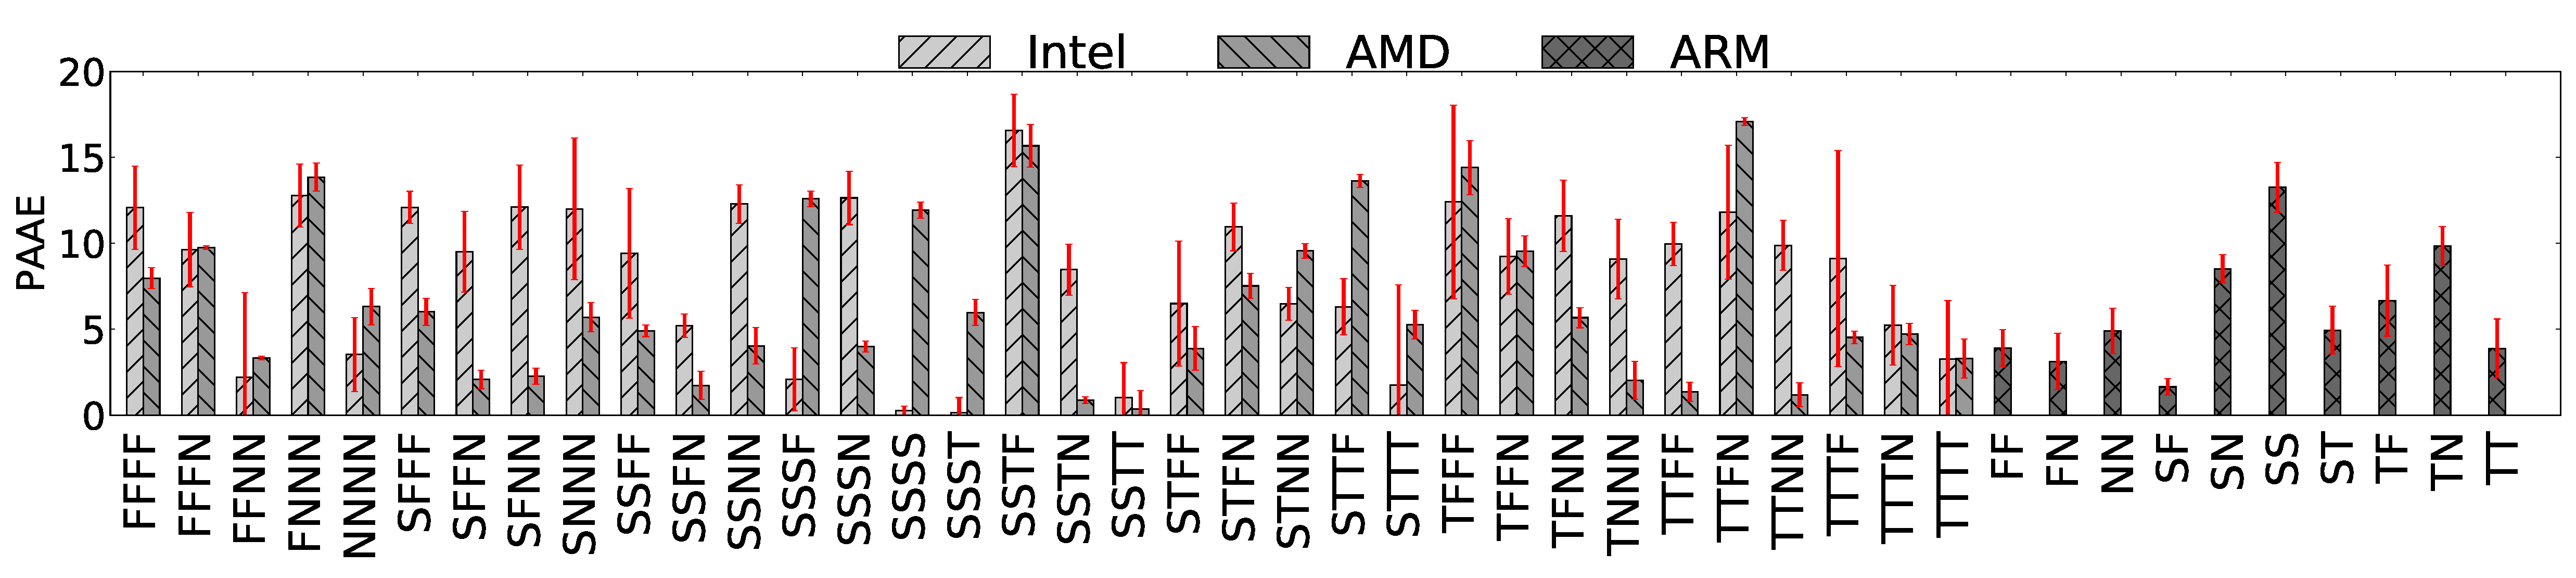
\includegraphics[width=\linewidth]{Chapter3/Figs/multicore/power-shorter-paae.eps}
        \caption{Power}
        \label{fig: power paae}
    \end{subfigure}
    \begin{subfigure}{\textwidth}
        \centering
        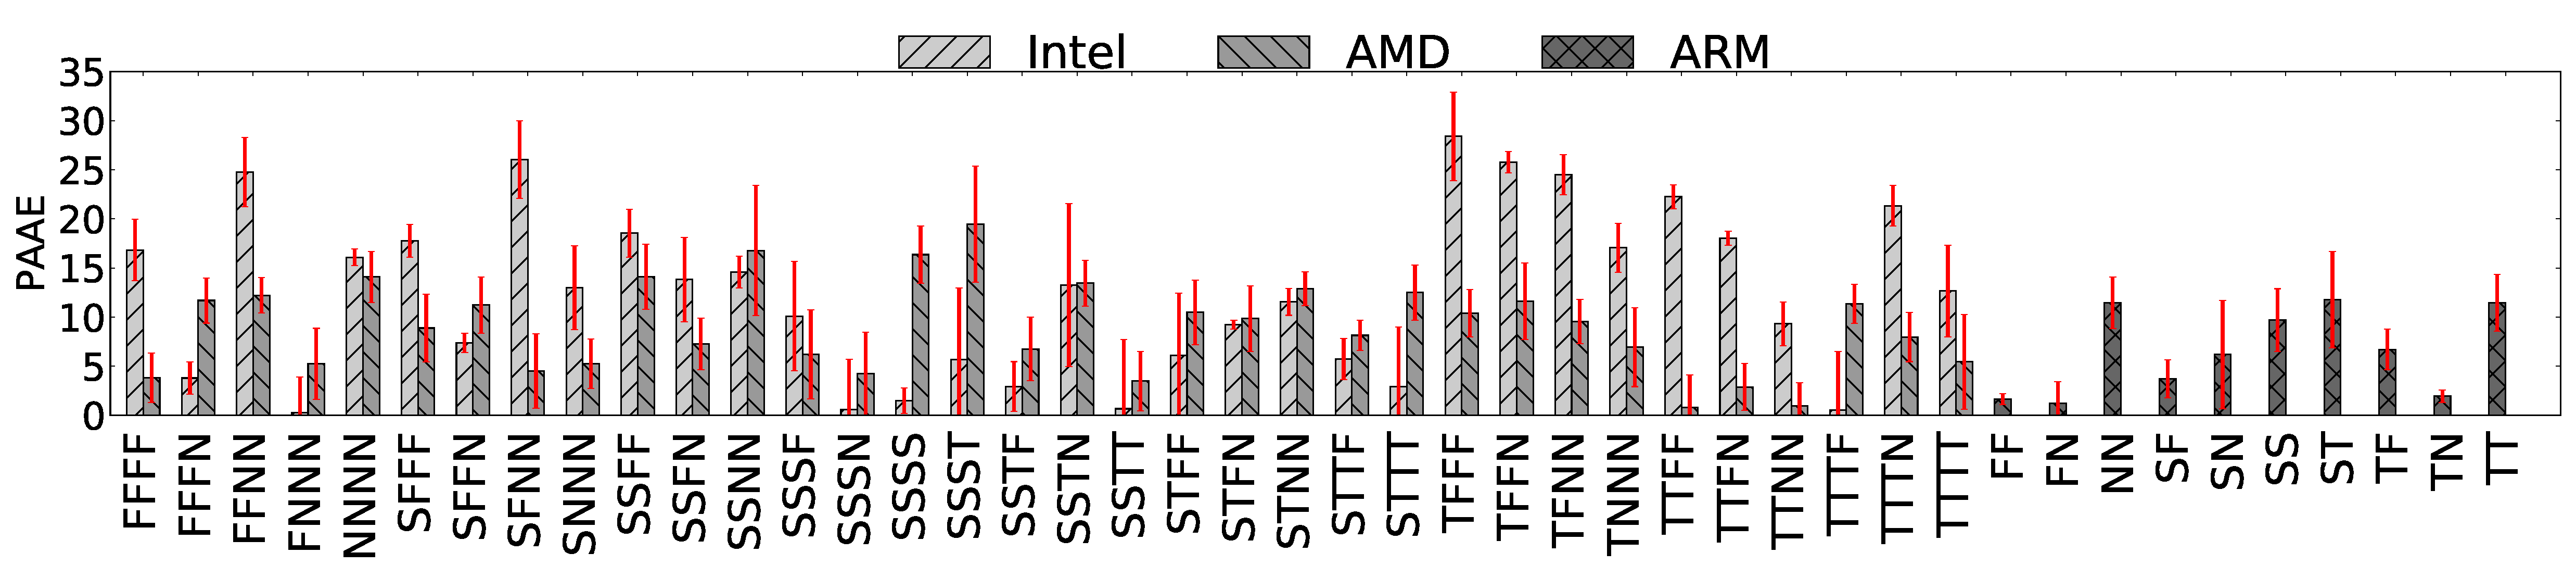
\includegraphics[width=\linewidth]{Chapter3/Figs/multicore/perf-shorter-paae.eps}
        \caption{Performance}
        \label{fig: perf paae}
    \end{subfigure} \caption[Average PAAE for REPP with multiple
    constraints]{\captitle{Average PAAE for REPP with multiple constraints.} Average
    PAAE when predicting power (\ref{fig: power paae}) and performance (\ref{fig: perf
    paae}) for all workloads under Low, Mid, High and Random change\_factors in multicore
    architectures. The error bars represent STDEV across change\_factors. The $x$-axis
    shows multiprogrammed workloads.} 
\label{fig: multicore result} 
\end{figure}

\looseness -1 Figure~\ref{fig: multicore result} shows the average PAAE for each workload when meeting
the performance (ARM \SI{7.1}{\percent}, AMD \SI{9.02}{\percent}, and Intel
\SI{7.1}{\percent}) and power (ARM \SI{6.0}{\percent}, AMD \SI{6.6}{\percent}, and Intel
\SI{8.1}{\percent}) requirements in ten experiments across architectures. The error bars
represent the STDEV across ten experiments for power and performance, which is less than
\SI{5.3}{\percent} for each workload. We focus on analysing those workloads with an error
greater than \SI{10}{\percent} in both architectures. When predicting power, we observe an
error of \SI{13.8}{\percent} (\SI{654.86}{\milli\joule}) on AMD for workload \texttt{FNNN}
that contains \emph{ep.C}, which has very high activity ratio in BPU (4.2542) and FE
(13.752).  Similarly for workload \texttt{TTFN}, Intel has a higher error
\SI{11.8}{\percent} (\SI{11.34}{\milli\joule}) than AMD, because on Intel we run two
instances of \emph{radix}, whereas on AMD we run a single one. Recall that the
multiprogrammed are generated based on the methodology described in
Section~\ref{subsection: batch workloads}, therefore we can not control  the number of
instances in a given workload. When predicting performance, we observe an error of 26.0\%
for \texttt{SFNN} on Intel because we run \emph{lu\_ncb}, which has non contiguous blocks
of memory and the activity ratio in LLC is higher relative to other benchmarks.
Similarly, workloads \texttt{TTTF} on AMD and \texttt{TTFN} on Intel have a power
prediction error of \SI{11.3}{\percent} and \SI{18.0}{\percent}, respectively, because
\emph{radix} is part of the multiprogrammed workloads.  The maximum performance error on
AMD, ARM and Intel are 19.4\% (769 MIPS for \texttt{SSST}), \SI{11.7}{\percent} (5389 MIPS
for \texttt{ST}) and \SI{28.4}{\percent} (13611 MIPS for \texttt{TFFF}). Similarly the
maximum power error AMD, ARM and Intel are \SI{17.0}{\percent} (\SI{101.72}{\milli\joule}
for \texttt{TTFN}), \SI{13.3}{\percent} (\SI{10}{\milli\joule} for \texttt{SS}) and
\SI{16.6}{\percent} (\SI{37.24}{\milli\joule} for \texttt{SSTF}), respectively. 

\begin{figure*}[tb!]
   \centering
    \begin{subfigure}{0.32\textwidth}
        \centering
        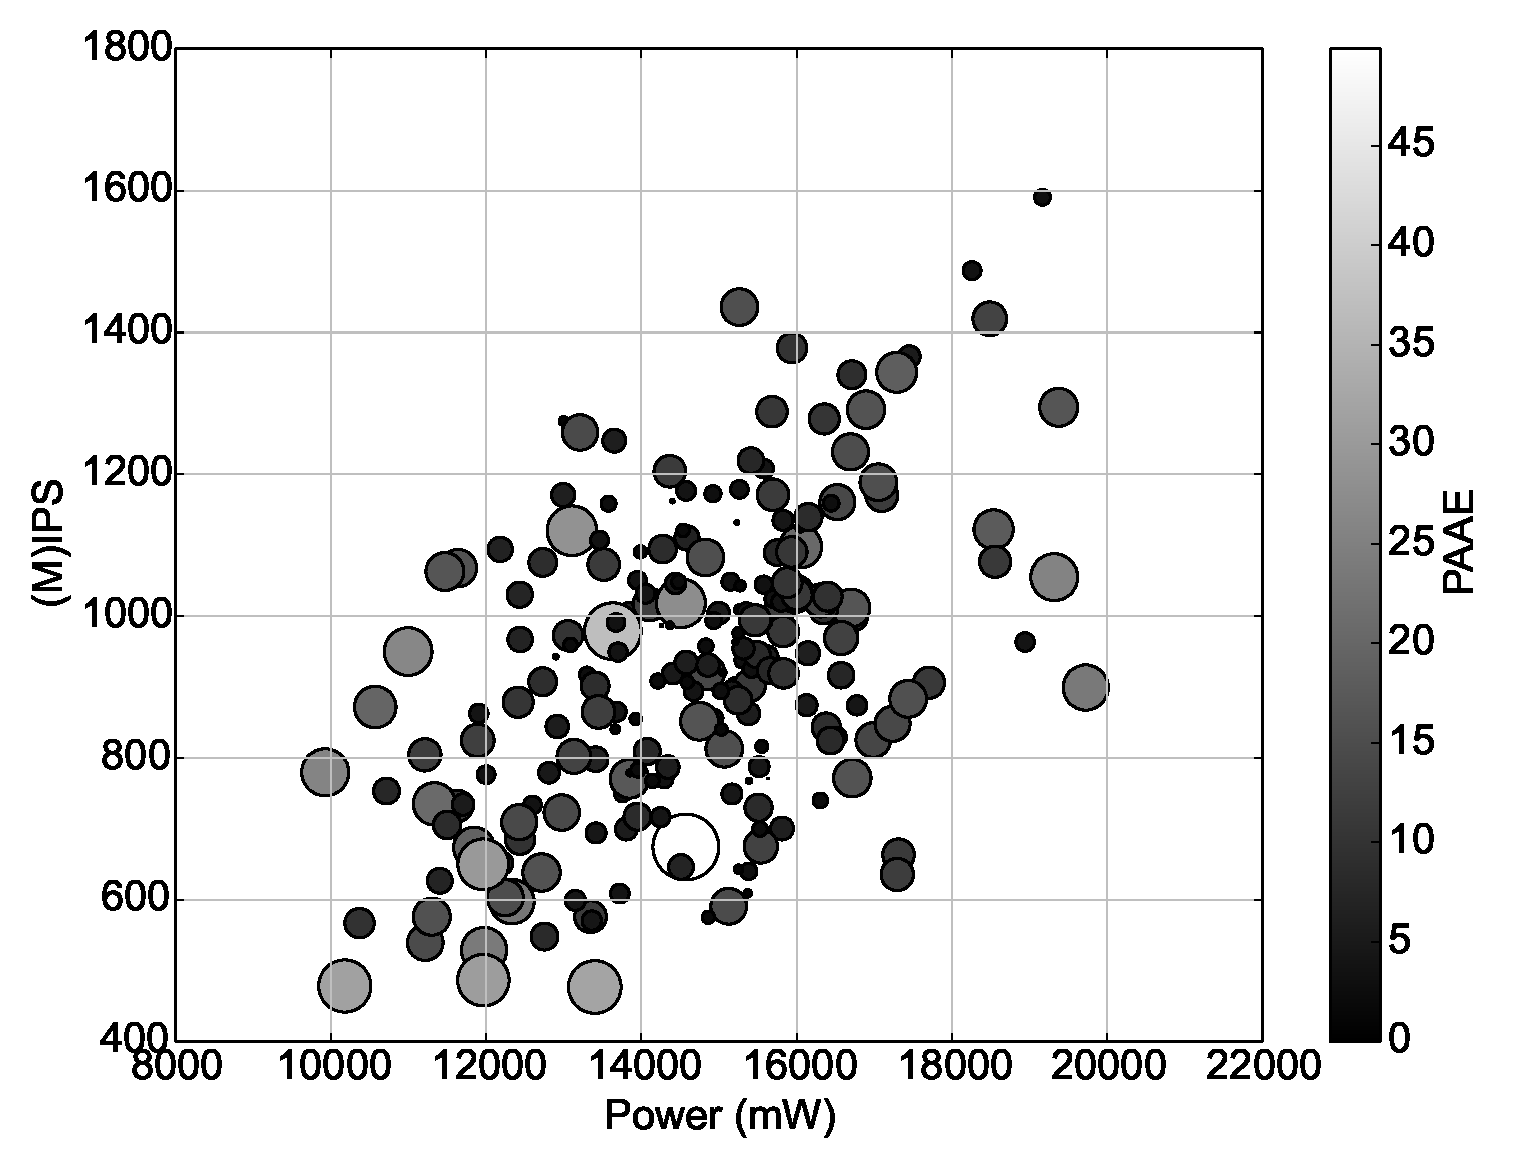
\includegraphics[width=\textwidth]{Chapter3/Figs/scatter/SSTN.eps}
        \caption{SSTN}
        \label{fig: SSTN}
    \end{subfigure}
    \begin{subfigure}{.32\textwidth}
        \centering
        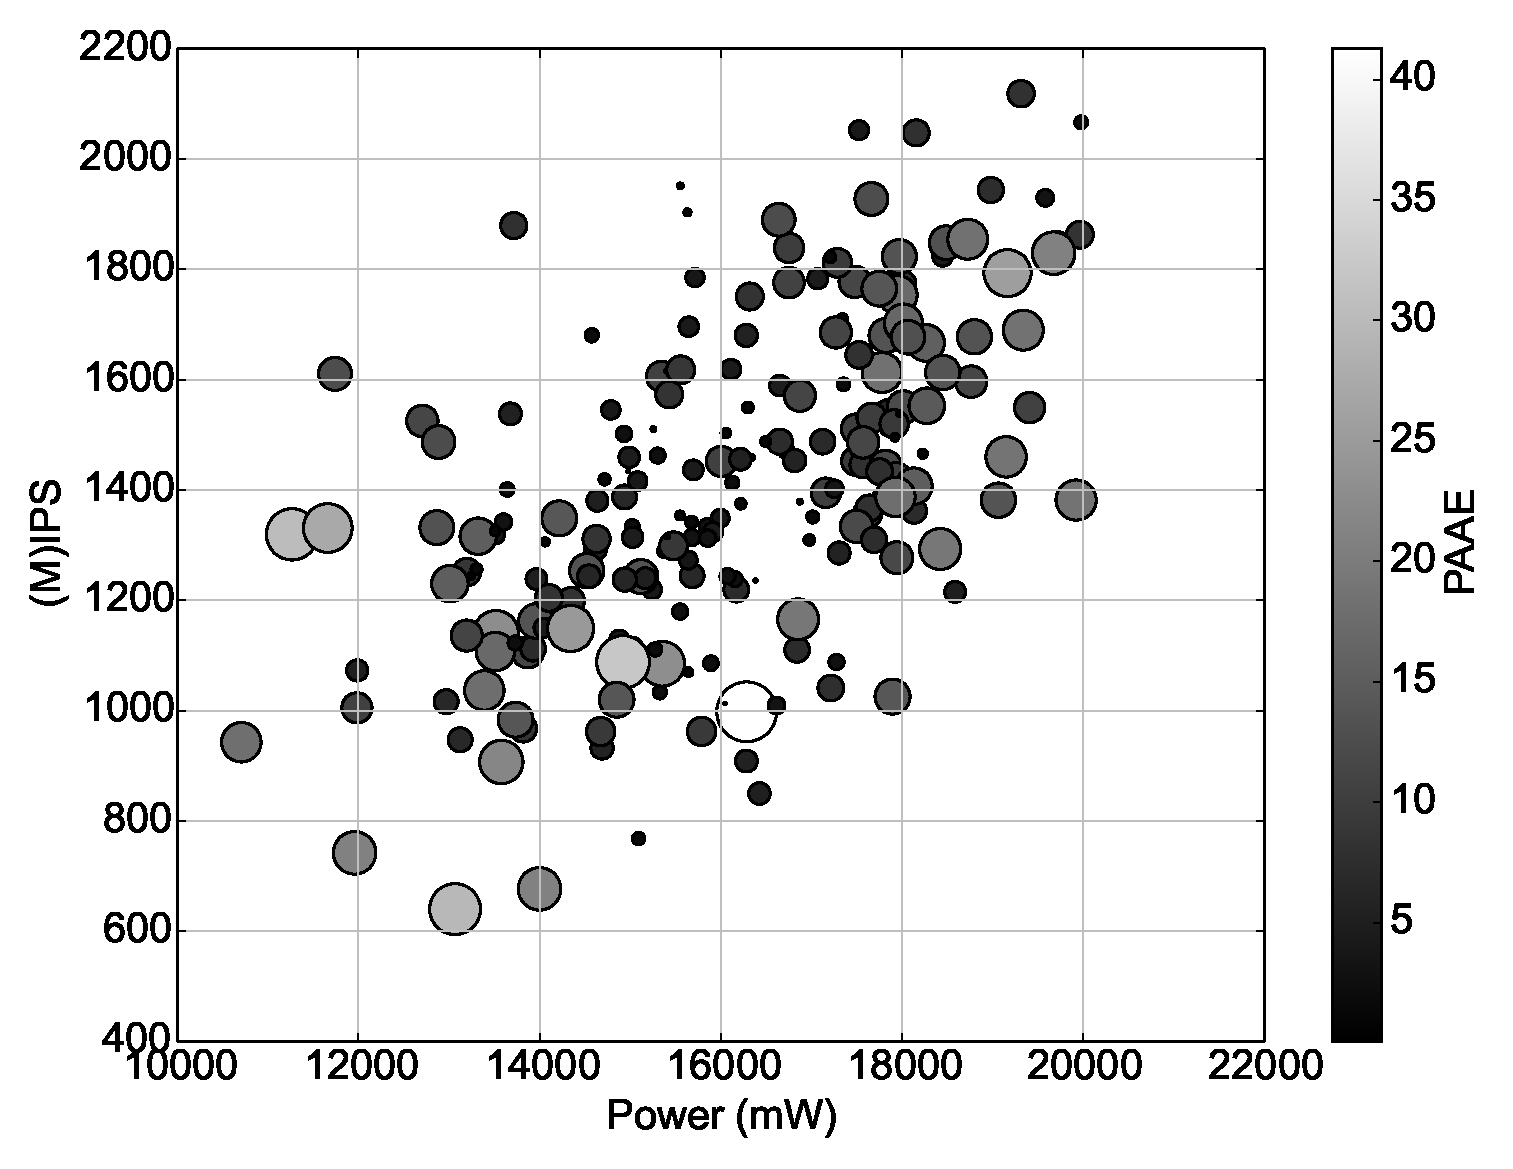
\includegraphics[width=\textwidth]{Chapter3/Figs/scatter/FFFN.eps}
        \caption{FFFN}
        \label{fig: FFFN}
    \end{subfigure}
    \begin{subfigure}{0.32\textwidth}
        \centering
        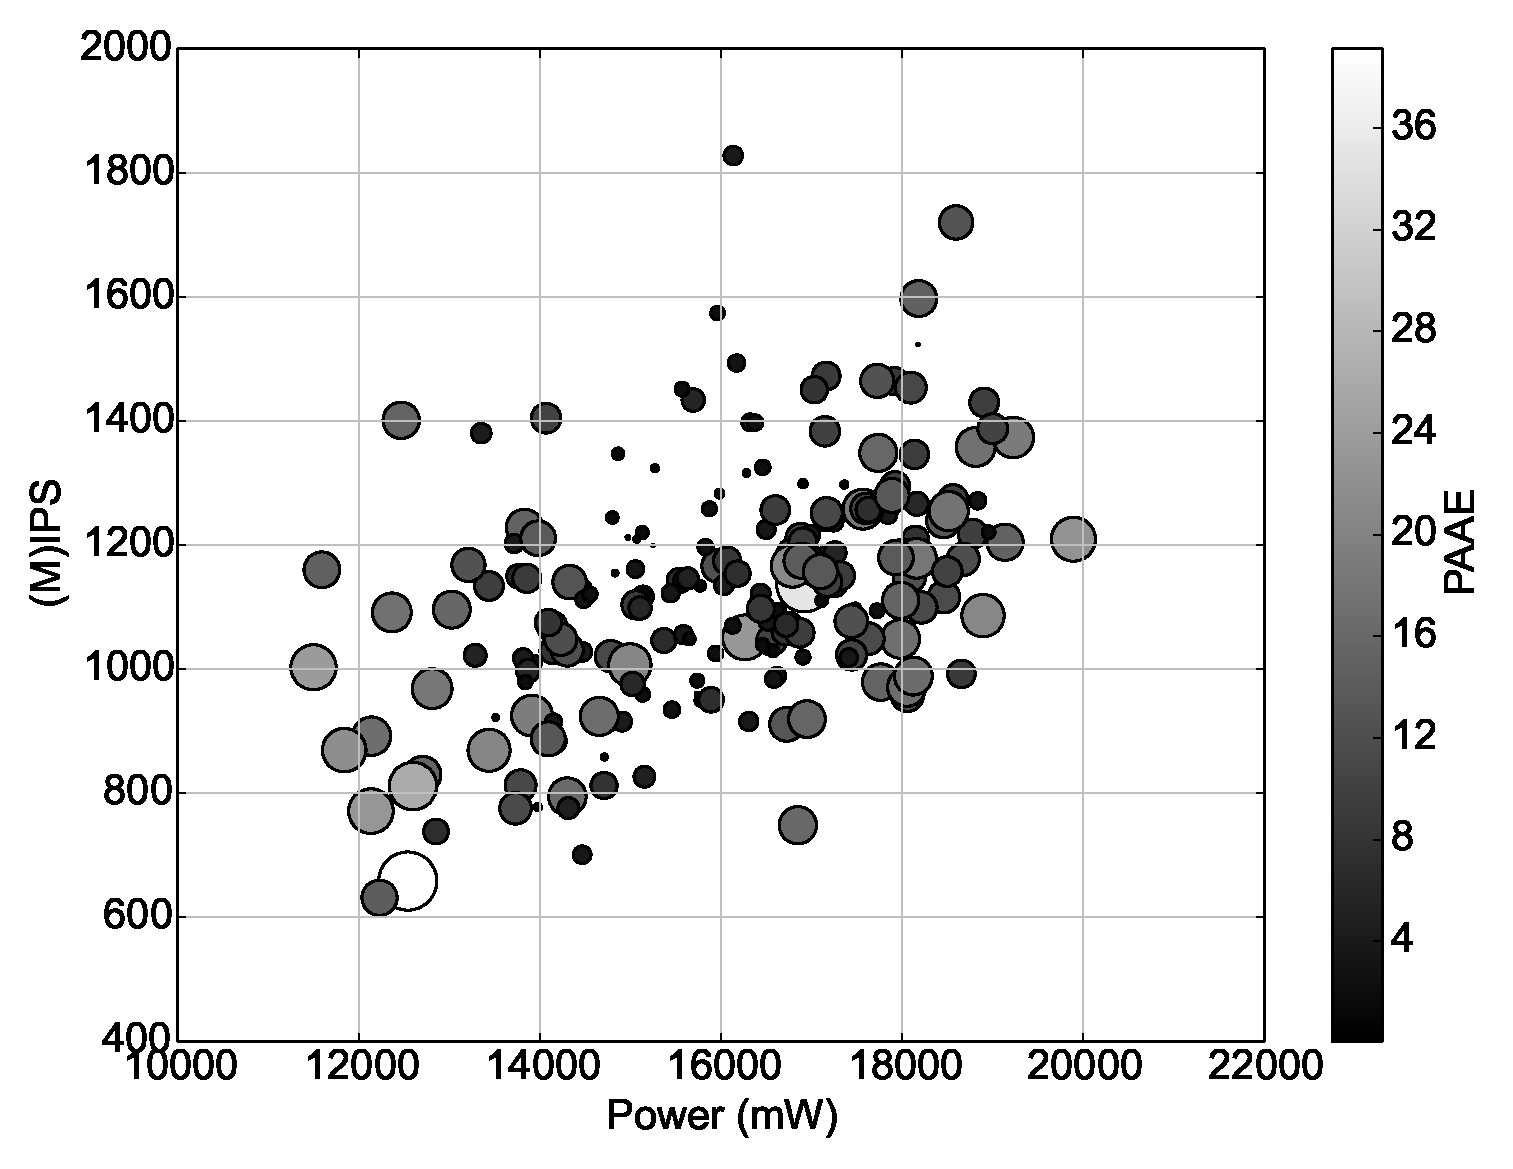
\includegraphics[width=\textwidth]{Chapter3/Figs/scatter/STFN.eps}
        \caption{STFN}  
        \label{fig: STFN}
    \end{subfigure}
    \caption[PAAE for workloads SSTN, FFFN and STFN on Intel]{\captitle{PAAE for workloads SSTN, FFFN and STFN on Intel.} Performance and power prediction error with change\_factor High.}
    \label{fig: REPPH result}
\end{figure*}

\looseness -1 Figure~\ref{fig: REPPH result} represents the performance on $y$-axis and
power on $x$-axis for multiprogrammed workloads SSTN, FFFN, and STFN on Intel architecture
with \textit{change\_factor} High. The radius of each circle is the maximum prediction
error, either power or performance (that is, $radius$ = $max$(PAAE\textsubscript{power},
PAAE\textsubscript{perf})). There exists multiple grayscale grading from low PAAE (black)
to high PAAE (white). Although the maximum PAAE shown is at the 50\% mark (the grayscale
in Figure~\ref{fig: SSTN} is up to 50\%), the number of error predictions with PAAE
greater than \SI{30}{\percent} is less than ten. For SSTN, FFFN and STFN, the average
error when predicting power (and performance) of \SI{9.7}{\percent} (\SI{3.3}{\percent}),
\SI{8.7}{\percent} (\SI{9.4}{\percent}) and \SI{8.4}{\percent} (\SI{6.7}{\percent}). This
behaviour is observed across all workloads.

\begin{figure}[t]
    \centering
    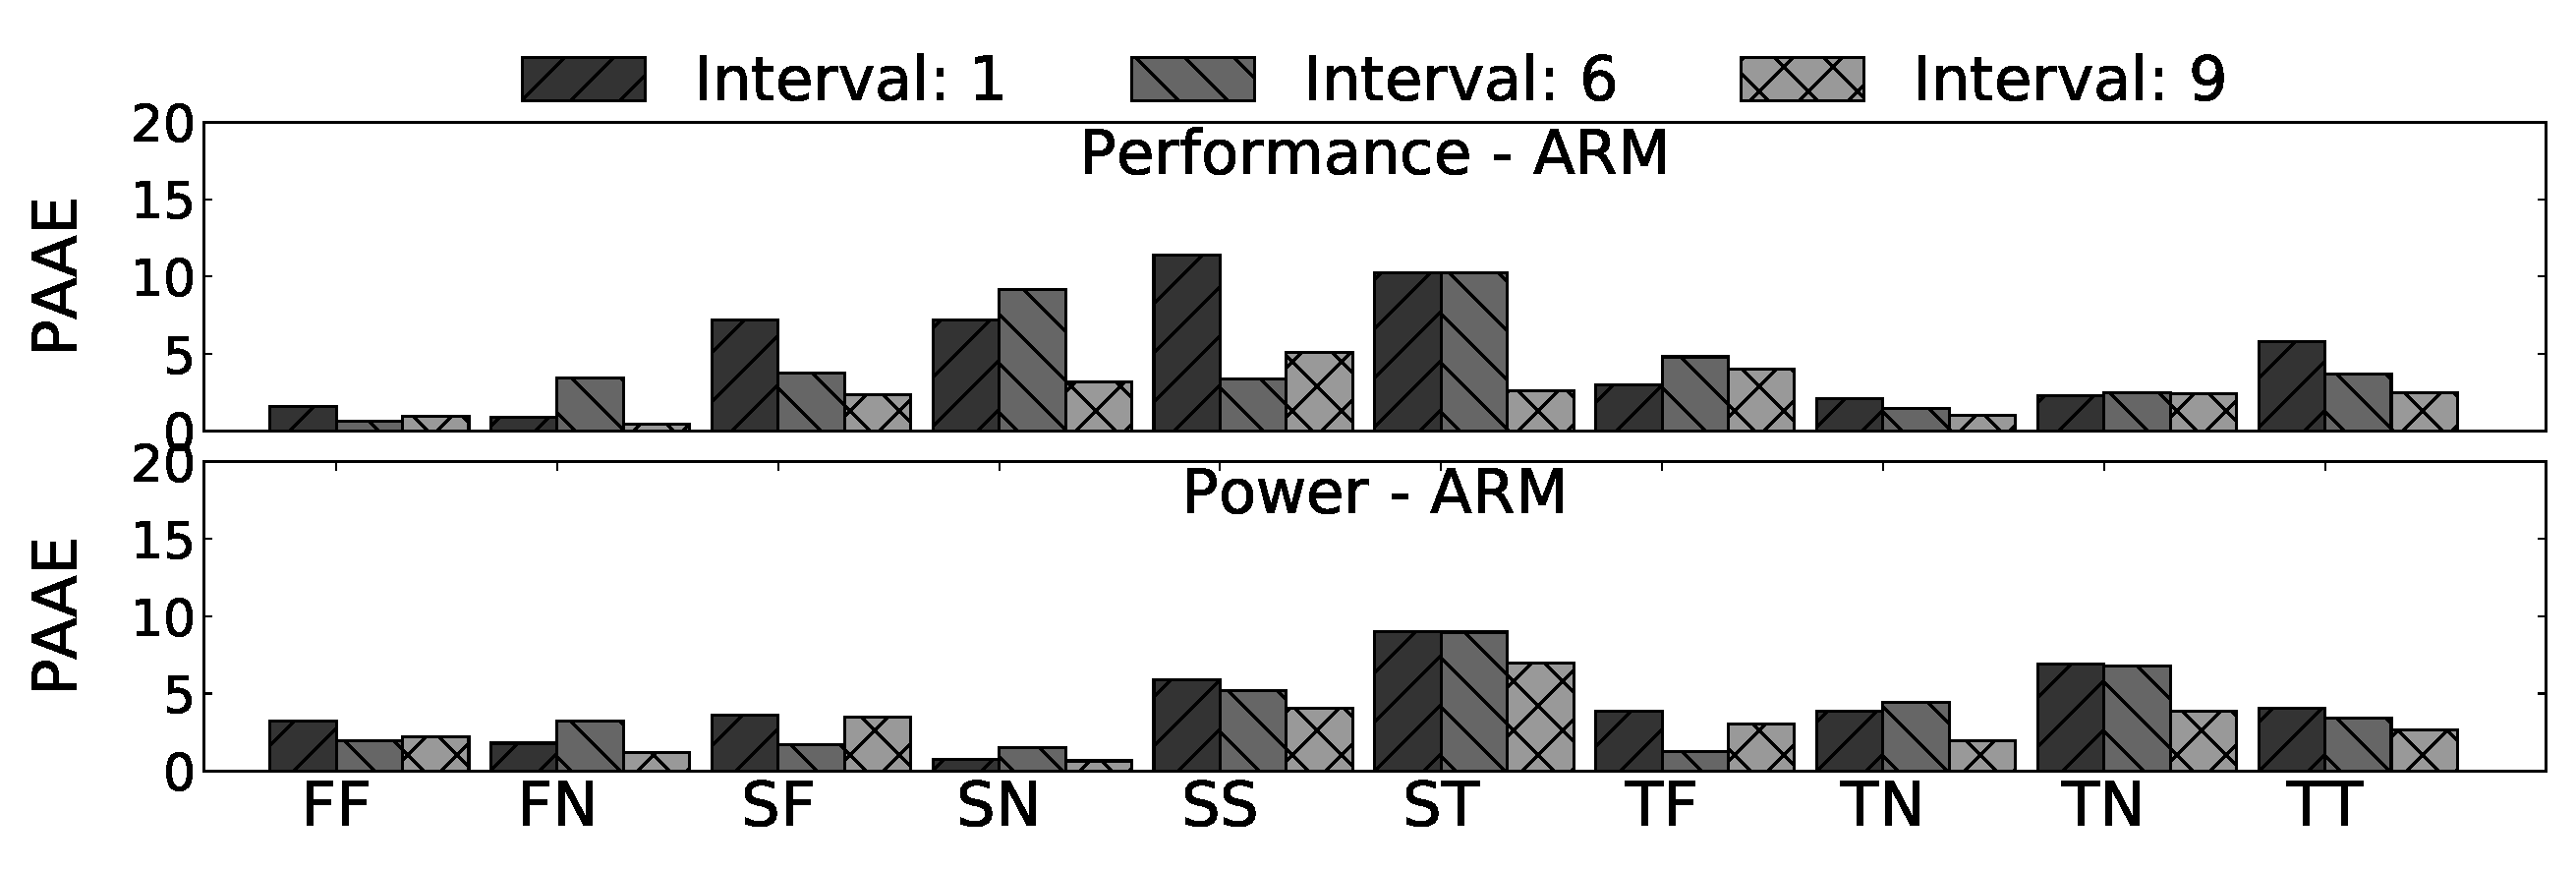
\includegraphics[width=\textwidth]{Chapter3/Figs/changefactor/summary-arm.eps}
    \caption[Average PAAE on ARM under different load\_change intervals]{\captitle{Average PAAE on ARM under different load\_change intervals.} Average PAAE when predicting power and performance for all workloads under different load\_change \texttt{intervals} for change\_factors Low, Mid and High. The $x$-axis shows multiprogrammed workloads.}
    \label{fig: armpowerperf}
\end{figure}

\begin{figure*}[htb!]
   \centering
    \begin{subfigure}{\textwidth}
        \centering
        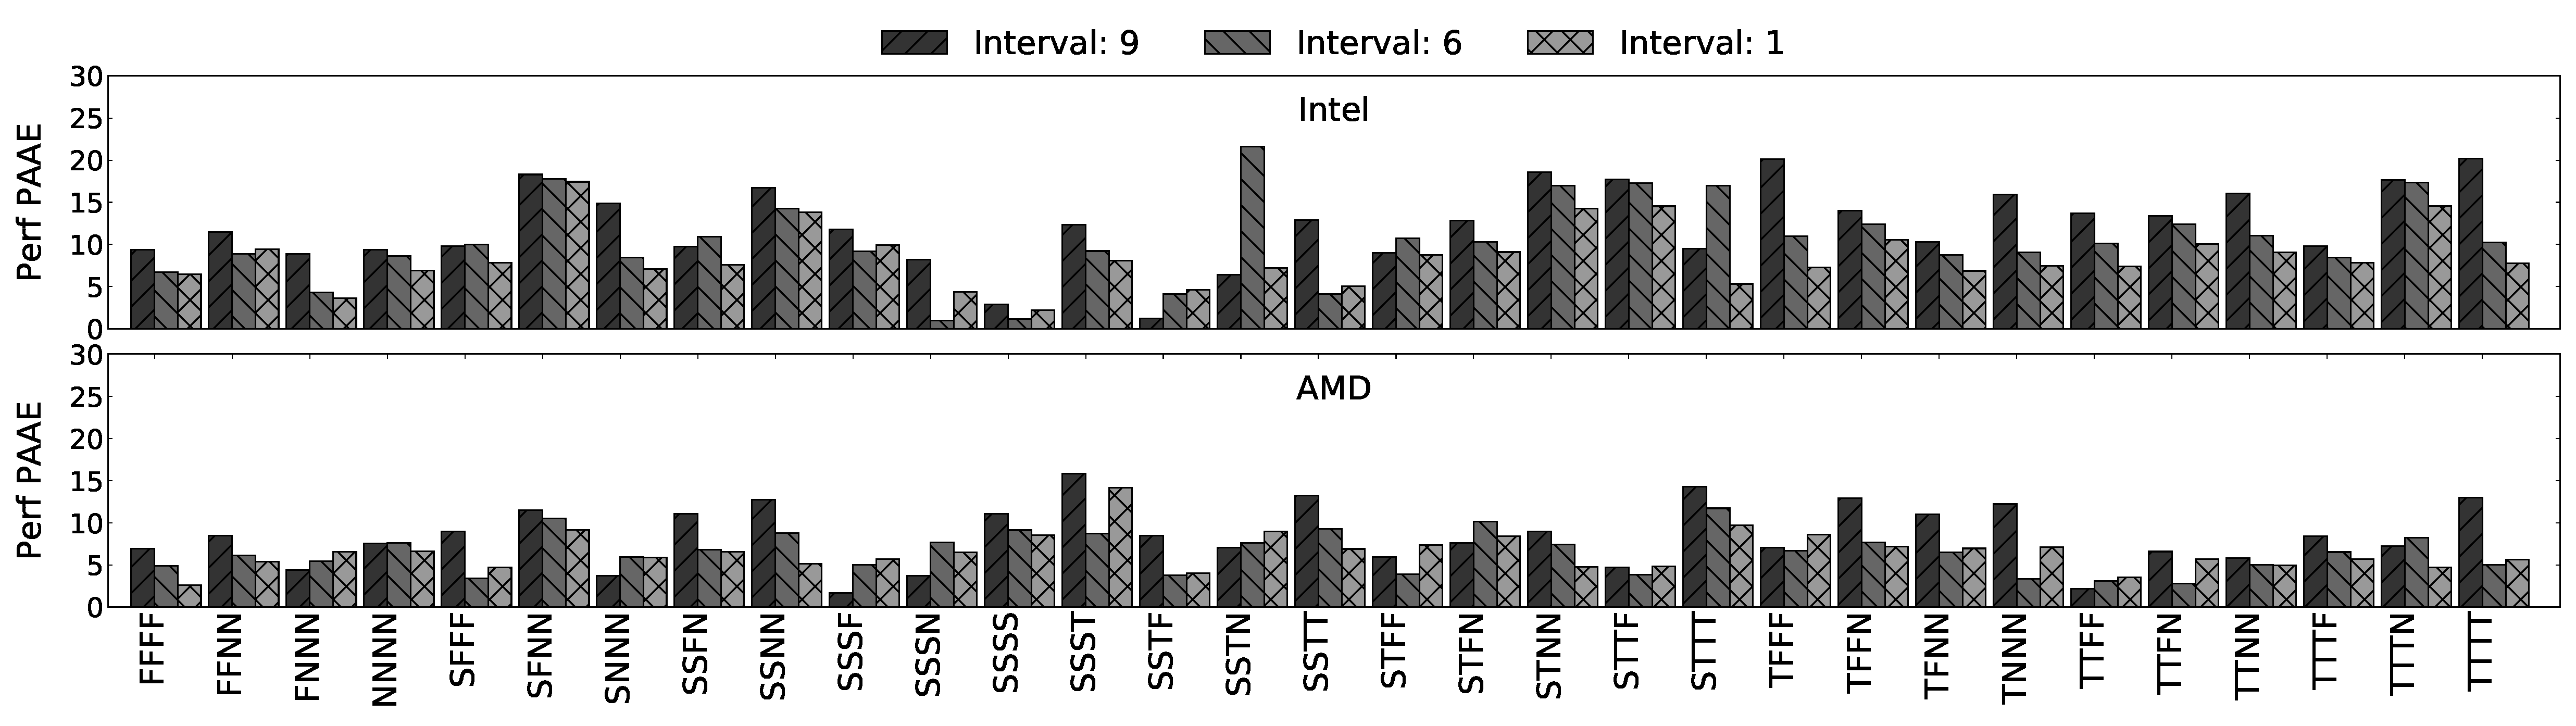
\includegraphics[width=\textwidth]{Chapter3/Figs/changefactor/summary_perf_intel_amd.eps}
        \caption{Performance}
        \label{fig: perfintelamd}
    \end{subfigure}
    \begin{subfigure}{\textwidth}
        \centering
        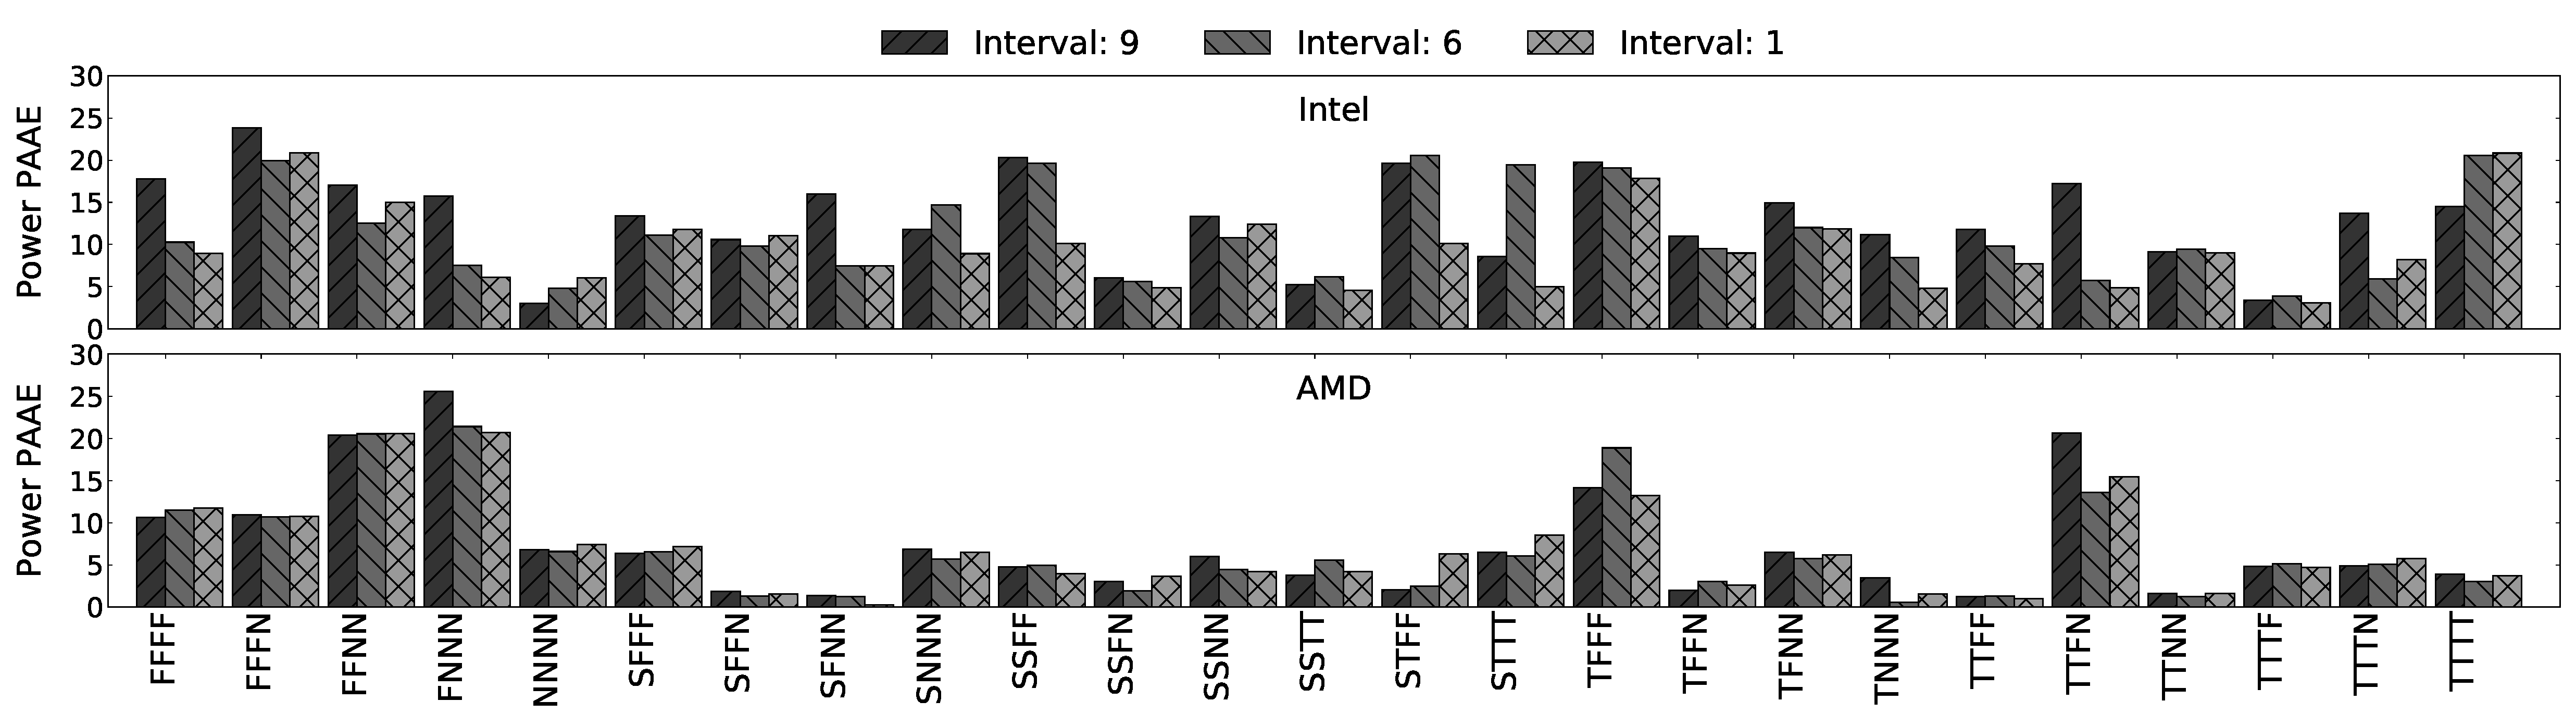
\includegraphics[width=\textwidth]{Chapter3/Figs/changefactor/summary_power_intel_amd.eps}
        \caption{Power}
        \label{fig: powerintelamd}
    \end{subfigure}
    \caption[Average PAAE on Intel and AMD under different load\_change intervals]{\captitle{Average PAAE on Intel and AMD under different load\_change intervals.} Average PAAE when predicting power and performance for all workloads under different load\_change \texttt{intervals} for change\_factors Low, Mid and High. The $x$-axis shows multiprogrammed workloads.}
    \label{fig: REPPH interval}
\end{figure*}


Figures~\ref{fig: REPPH interval} and~\ref{fig: armpowerperf} show the average PAAE for
each workload under different load\_change \texttt{intervals} on ARM and Intel/AMD when
predicting performance (Figure~\ref{fig: perfintelamd}) and power (Figure~\ref{fig:
powerintelamd}). Figures~\ref{fig: armpowerperf} and~\ref{fig: REPPH interval} are
separated because ARM has different number of cores. Across the three architectures,
faster (interval=1) load\_changes have \SI{3.5}{\percent} higher error compared to slower
(interval=9) load\_changes because of aggressive changes in load in short burst cause
numerous changes in configuration, thus leading to a higher error. On the other hand,
slower load\_changes lead to fewer changes in configuration, and have stable phases in
application behaviour.  Fortunately, data centres seldom want to jump from \SI{400}{\watt}
to \SI{600}{\watt} every second~\citep{6008553, Su:2014:POP:2742155.2742200}.
Table~\ref{tab: summarytable} summarises the result obtained when predicting power and
performance for load\_change interval \SI{1}{\second}, \SI{6}{\second} and
\SI{9}{\second}.

\begin{table}[ht]
\centering
\caption[Average PAAE for load\_change intervals]{\captitle{Average PAAE for load\_change intervals.} Power and performance error for load\_change intervals 1, 6 and 9 on Intel, AMD, and ARM.}
\begin{tabular}{@{}rrrrcrrrc@{}}\toprule
& \multicolumn{3}{c}{$Power$} & \phantom{abc}& \multicolumn{3}{c}{$Performance$} & \phantom{abc} \\
\cmidrule{2-4} \cmidrule{6-8} 
    $Interval$ & $\SI{1}{\second}$ & $\SI{6}{\second}$ & $\SI{9}{\second}$ && $\SI{1}{\second}$ & $\SI{6}{\second}$ & $\SI{9}{\second}$ \\ 
\midrule
    $Intel$     & \SI{11.1}{\percent} & \SI{7.3}{\percent}    & \SI{5.6}{\percent}  && \SI{11.4}{\percent} & \SI{10.6}{\percent}   & \SI{8.7}{\percent} \\
    $AMD$       & \SI{7.2}{\percent}  & \SI{6.9}{\percent}    & \SI{6.7}{\percent}  && \SI{8.5}{\percent}  & \SI{6.5}{\percent}    & \SI{6.5}{\percent} \\
    $ARM$       & \SI{4.2}{\percent} & \SI{3.8}{\percent}     & \SI{2.9}{\percent}  && \SI{5.1}{\percent}  & \SI{4.6}{\percent}    & \SI{2.4}{\percent} \\
\bottomrule
\end{tabular}
\label{tab: summarytable}
\end{table}

%\vspace*{2em}

\paragraph{Enabling Power/Performance Capping.} Determining a configuration to meet the
minimum performance (or not exceeding power consumption threshold) is usually done in an
iterative fashion (as in the RAPL driver on Intel processors~\citep{Intel}). A feedback
control loop is often used to determine the  configuration. If the power usage is above a
certain threshold, the configuration is lowered. On the other hand, if the power usage is
below a certain threshold, the configuration is increased to improve performance. In
contrast, we provide a single-step mechanism to select configurations.

\begin{figure}[t]
    \centering
    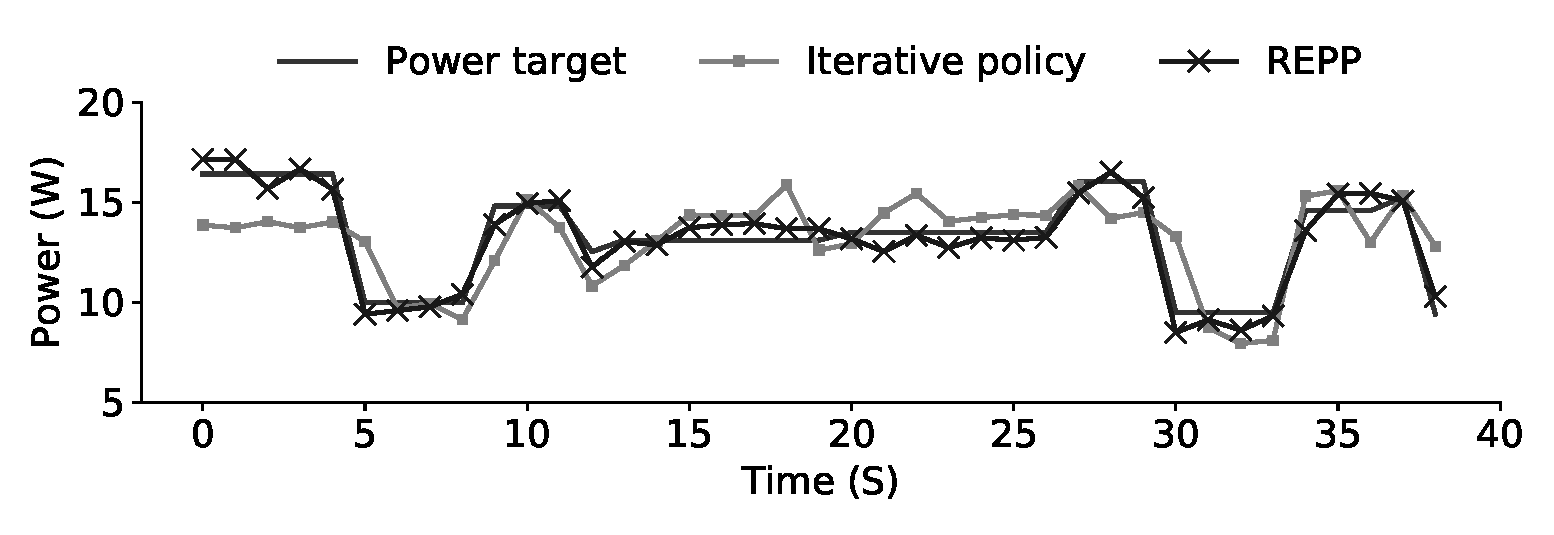
\includegraphics[width=\textwidth]{Chapter3/Figs/runtime/intel-runtime.eps}
    \caption[Responsiveness to power change on Intel]{\captitle{Responsiveness to power change on Intel.} Responsiveness to power capping for workload SSTT with constraint Random.}
    \label{fig: SSTT}
\end{figure}

Figure~\ref{fig: SSTT} shows the responsiveness to (dynamic) power capping for workload
\texttt{SSTT}, where the power capping limit is Random on Intel platform in the first 40
seconds. \texttt{SSTT} is composed of applications \emph{streamcluster}, \emph{lu.C},
\emph{bwaves} and \emph{soplex}. REPP changes DVFS states and meets the power target in
0.37 seconds on average, which is 3.6$\times$  faster than the iterative algorithm (used
by Intel RAPL). This time includes sampling interval, latency to predict at all DVFS state
and Cl-State and time to change DVFS state.  Moreover REPP, provides \SI{6}{\percent}
higher prediction accuracy. 

